\section{Big Data Analytics - II Lecture}

\subsection{Introduction to Big Data}

Good morning, class. Today, we will be discussing the concept of big
data and its magnitude. To begin, let me share my screen so we can dive
into the presentation slides. Now, the question that naturally arises
is: how big is big data?

\subsection{The Rise of Big Data}

\subsubsection{Global Data Growth}

\begin{figure}[!h]
    \centering
    \includegraphics[page=26, trim = 1.3cm 0.7cm 1.5cm 3.5cm, clip, width=\textwidth]{images/06 - BIG_DATA.pdf}
\end{figure}

The rise of big data is a result of two main factors: the exponential
increase in the amount of data produced globally and the shift from
analog to digital support. If we consider big data as the vast amount of
information produced globally on any type of support, we can see from a
chart sourced from Wikipedia that there has been a significant increase
in data production since around 2002. This coincides with the beginning
of the digital age, marked by the widespread adoption of the internet
and the subsequent emergence of social media platforms. The global
connectivity facilitated by these technological advancements has led to
a surge in the sheer volume of information generated. Additionally,
there has been a transition from analog support, such as tapes, to
digital support, further contributing to the growth of big data.

\subsubsection{Digital Age and Data Explosion}

\begin{figure}[!h]
    \centering
    \includegraphics[page=27, trim = 1.5cm 2cm 1.5cm 3.5cm, clip, width=\textwidth]{images/06 - BIG_DATA.pdf}
\end{figure}

In terms of quantity, the executive chairman of Google has provided a
striking summary of these trends. He noted that from the beginning of
human civilization until 2003, we generated a total of five exabytes of
data. However, currently, we are producing the same amount of data, five
exabytes, every two days, and this rate is increasing rapidly. This
global perspective aligns with the information presented in the chart we
just reviewed on Wikipedia.

\subsection{Understanding Data Units}

\subsubsection{Data Measurement Units}

But from a business perspective, do we really need to talk about
exabytes when discussing big data? Let's start with a brief summary of
what exabytes are. The units of data measurement range from kilobyte to
zettabyte, with kilobyte, megabyte, gigabyte, terabyte, petabyte, and
exabyte in between. You're probably familiar with gigabytes and
megabytes because you can typically store up to one terabyte of data on
your laptop's hard drive. So you have a general understanding of what a
terabyte is and how much information it can hold. To put it in
perspective, one thousand terabytes make up a petabyte, one thousand
petabytes make up an exabyte, and one thousand exabytes make up a
zettabyte.

\subsubsection{Forecast of IP Traffic}

\begin{figure}[!h]
    \centering
    \includegraphics[page=28, trim = 1.5cm 4.3cm 1.5cm 3.8cm, clip, width=\textwidth]{images/06 - BIG_DATA.pdf}
\end{figure}

To better understand the trends we are discussing, it is forecasted that
IP traffic will reach three zettabytes per year by the end of 2021. It's
important to note that this is still a forecast and the actual data is
not yet available. Zettabytes, along with exabytes, are significant
units of measurement in this context.

\subsection{Defining Big Data}

\begin{figure}[!h]
    \centering
    \includegraphics[page=29, trim = 1.5cm 6.5cm 1.5cm 4.5cm, clip, width=\textwidth]{images/06 - BIG_DATA.pdf}
\end{figure}

\subsubsection{Business Perspective}

Before we can discuss the technical aspects and requirements of big
data, it is important to define what exactly big data is from a business
perspective. While some may argue that terabytes of data are not
sufficient to be considered big data, it is crucial to understand that
the size of the data alone does not determine its classification. To
provide a practical answer to this question, let's refer to Forbes'
definition of big data, which states that it is \textit{a collection of data
    from both traditional and digital sources, both within and outside an
    organization}. This data serves as a valuable resource for ongoing
discovery and analysis.

What stands out in this definition is the close relationship between big
data and analysis. The true essence of big data lies in its ability to
be analyzed and interpreted for meaningful insights.

\subsubsection{Technical Scalability Challenges}

Big data and analytics are closely intertwined and often referred to
together as ``big data analytics.'' Big data refers to a large volume of
data that can provide valuable insights when analyzed. From a technical
perspective, big data is any amount of data that presents scalability
challenges during analysis. Even relatively small datasets can pose
technical scalability issues depending on the type of analytics being
performed. In fact, even a few gigabytes of data can be considered big
data for certain types of analytics. Terabytes of data are certainly
considered big data, even if they can be stored on a laptop's hard
drive.

Analyzing terabytes of data can be a challenging task. Just think about
how long it takes to back up the data on your hard drive, which can
require hours for just a few hundred gigabytes. This highlights the
technical challenges that arise when building interactive applications
that require fast response times but involve transferring relatively
small amounts of data.

While industrial systems are more powerful than laptops, it's important
to recognize that as data size grows, time becomes a significant factor
in both personal and business contexts. This is especially true for
enterprise technologies.

\subsection{Classification of Data Types}

\begin{figure}[!h]
    \centering
    \includegraphics[page=30, trim = 1.5cm 1.7cm 2cm 4.5cm, clip, width=\textwidth]{images/06 - BIG_DATA.pdf}
\end{figure}

Now, let's take a closer look at the different types of data and their
sizes within the realm of big data. We can classify the data into
various categories, such as conversation text data from platforms like
Twitter and Facebook, photo and video image data from platforms like
YouTube, audio files from call centers, sensor data like seismic or
satellite data, Internet of Things (IoT) data collected from smart
devices and smartphones, web customer data including web logs that track
customer actions on websites, and traditional customer data like
receipts, loyalty programs, and traffic data from telephone and internet
operators.

\subsubsection{Conversation Text Data}

To give you an idea of the scale of these data types, let's start with
conversation text data from Twitter and Facebook. On average, around
6,000 tweets are posted every second on Twitter. If we focus solely on
text-based tweets and exclude images and videos, this amounts to
approximately 200 billion tweets per year, equivalent to 25 terabytes of
data annually.

\subsubsection{Photo and Video Image Data}

Analyzing data may seem like a small task, but it becomes significant
when dealing with large amounts of information. For instance, if you use
a semantic engine to process text data, it can take approximately one
day to process one megabyte on a single core of a server. This means
that analyzing 25 terabytes of data would require a substantial amount
of time. It's important to note that the amount of data goes beyond just
Twitter; there are also 152 million blogs, Facebook, and even text data
from YouTube. Additionally, image, audio, and video data are even larger
in size. While text data is measured in terabytes, a JPEG picture can
range from one to six megabytes, depending on its quality. On Facebook
alone, this adds up to approximately 120 petabytes of pictures per year.

\subsubsection{Audio Files}

When it comes to audio recordings, the amount of data can quickly reach
petabytes. In the context of a call center, where an average
conversation is about 20 megabytes, and the center handles around 1000
calls per day, recording all calls would result in approximately 1.3
gigabytes of data per day. This adds up to half a terabyte of audio
recordings per year. Therefore, the volume of audio data is still in the
terabytes range.

\subsubsection{Sensor Data}

When it comes to video data, the size can quickly add up. High-quality
video typically takes up around 100 megabytes per minute, and on
platforms like YouTube, this amounts to a staggering 2.5 petabytes per
day. This demonstrates the immense volume of data involved.

However, sensor data presents an even more challenging scenario. Sensors
have the capability to record audio, capture images, and even record
videos. They can also combine different types of data, such as photos
with related text or videos with audio streams. Sensor data is collected
continuously and can easily accumulate to the petabyte scale. For
instance, a video surveillance service alone can generate one petabyte
of data in just five days.

\subsubsection{Internet of Things Data}

Typically, video surveillance services do not store their data for
extended periods of time. They record videos but eventually delete them.
On the other hand, the Internet of Things (IoT) is rapidly expanding,
with 26 billion units installed in 2020 and counting. The IoT generates
a significant amount of data, producing approximately 10 petabytes per
year if each unit generates one kilobyte of text daily. This amount is
equivalent to 40 times the text data produced by Twitter and Facebook
combined. It's important to note that the IoT data also includes photos,
audio, and video, which further contributes to the overall data volume,
easily reaching the petabyte scale.

\subsubsection{Web Customer Data}

In practice, companies often transfer streaming data to a central
location where it is processed and only a summary of the IoT data is
permanently stored. This approach is both economically and technically
feasible. For example, web customer data in a log file is not large,
typically ranging from 250 to 750 bytes. However, when accumulated over
time, it can add up to 7.5 megabytes per day for a single site. At an
enterprise level, this can reach several gigabytes per day, resulting in
a few terabytes per year.

To manage this data size, organizations do not store all the data
indefinitely. Instead, they retain it for a certain period of time and
then apply log file rotation on a daily, weekly, or monthly basis. This
means that even a few terabytes per year prompts companies to implement
data lifecycle management, periodically deleting data to avoid exceeding
a certain threshold of permanently stored data.

\subsubsection{Traditional Customer Data}

Traditional customer data refers to the data collected from customers in
a business context. The size of this data can vary depending on the type
and size of the business, ranging from 0.5 to 10 terabytes per year when
compressed. The largest component of traditional customer data is
transaction information, which is crucial in an enterprise context.

While this amount of data may not seem significant, it becomes more
substantial when considering industries like banking. Banks are required
to retain transaction data for an extended period, typically up to 10
years. As a result, banks accumulate a large volume of data over time.
For example, an Italian bank would have slightly less than a petabyte of
data in total.

\subsection{Big Data in Practice}

Although traditional relational technologies can handle large data
sizes, they are not efficient when it comes to data analytics and
analysis. This is mainly due to factors such as data normalization,
which ensures correctness and consistency but hampers fast data access.
So, while traditional technologies are suitable for managing data, they
are slow when it comes to analyzing it.

In the next class, we will explore how SQL technologies have evolved to
address the challenges of big data. We will learn about more efficient
tools and techniques that can be used to handle big data projects.
